\documentclass[a4paper,
fontsize=11pt,
%headings=small,
oneside,
numbers=noperiodatend,
parskip=half-,
bibliography=totoc,
final
]{scrartcl}

\usepackage[babel]{csquotes}
\usepackage{synttree}
\usepackage{graphicx}
\usepackage{accessibility}

\setkeys{Gin}{width=.4\textwidth} %default pics size

\graphicspath{{./plots/}}
\usepackage[english]{babel}
\usepackage[T1]{fontenc}
%\usepackage{amsmath}
\usepackage[utf8x]{inputenc}
\usepackage [hyphens]{url}
\usepackage{booktabs} 
\usepackage[left=2.4cm,right=2.4cm,top=2.3cm,bottom=2cm,includeheadfoot]{geometry}
\usepackage[labelformat=empty]{caption} % option 'labelformat=empty]' to surpress adding "Abbildung 1:" or "Figure 1" before each caption / use parameter '\captionsetup{labelformat=empty}' instead to change this for just one caption
\usepackage{eurosym}
\usepackage{multirow}
\usepackage[ngerman]{varioref}
\setcapindent{1em}
\renewcommand{\labelitemi}{--}
\usepackage{paralist}
\usepackage{pdfpages}
\usepackage{lscape}
\usepackage{float}
\usepackage{acronym}
\usepackage{eurosym}
\usepackage{longtable,lscape}
\usepackage{mathpazo}
\usepackage[normalem]{ulem} %emphasize weiterhin kursiv
\usepackage[flushmargin,ragged]{footmisc} % left align footnote
\usepackage{ccicons} 
\setcapindent{0pt} % no indentation in captions
\usepackage{xurl} % Breaks URLs

%%%% fancy LIBREAS URL color 
\usepackage{xcolor}
\definecolor{libreas}{RGB}{112,0,0}

\usepackage{listings}

\urlstyle{same}  % don't use monospace font for urls

\usepackage[fleqn]{amsmath}

%adjust fontsize for part

\usepackage{sectsty}
\partfont{\large}

%Das BibTeX-Zeichen mit \BibTeX setzen:
\def\symbol#1{\char #1\relax}
\def\bsl{{\tt\symbol{'134}}}
\def\BibTeX{{\rm B\kern-.05em{\sc i\kern-.025em b}\kern-.08em
    T\kern-.1667em\lower.7ex\hbox{E}\kern-.125emX}}

\usepackage{fancyhdr}
\fancyhf{}
\pagestyle{fancyplain}
\fancyhead[R]{\thepage}

% make sure bookmarks are created eventough sections are not numbered!
% uncommend if sections are numbered (bookmarks created by default)
\makeatletter
\renewcommand\@seccntformat[1]{}
\makeatother

% typo setup
\clubpenalty = 10000
\widowpenalty = 10000
\displaywidowpenalty = 10000

\usepackage{hyperxmp}
\usepackage[colorlinks, linkcolor=black,citecolor=black, urlcolor=libreas,
breaklinks= true,bookmarks=true,bookmarksopen=true]{hyperref}
\usepackage{breakurl}

%meta
%meta

\fancyhead[L]{A. Struck\\ %author
LIBREAS. Library Ideas, 45 (2024). % journal, issue, volume.
\href{https://doi.org/10.18452/29141}{\color{black}https://doi.org/10.18452/29141}
{}} % doi 
\fancyhead[R]{\thepage} %page number
\fancyfoot[L] {\ccLogo \ccAttribution\ \href{https://creativecommons.org/licenses/by/4.0/}{\color{black}Creative Commons BY 4.0}}  %licence
\fancyfoot[R] {ISSN: 1860-7950}

\title{\LARGE{Library Music – Audio for the Screens from Libraries of Sound}}% title
\author{Alexander Struck} % author

\setcounter{page}{1}

\hypersetup{%
      pdftitle={Library Music – Audio for the Screens from Libraries of Sound},
     pdfauthor={Alexander Struck},
      pdfcopyright={CC BY 4.0 International},
      pdfsubject={LIBREAS. Library Ideas, 45 (2024).},
      pdfkeywords={music, library, production music, stock music, rights, graphic design, Musik, Bibliothek, Produktionsmusik, Rechte, Grafikdesign},
      pdflicenseurl={https://creativecommons.org/licenses/by/4.0/},
      pdfurl={https://doi.org/10.18452/29141},
      pdfdoi={10.18452/29141},
      pdflang={en},
      pdfmetalang={en}
     }



\date{}
\begin{document}

\maketitle
\thispagestyle{fancyplain} 

%abstracts
\begin{abstract}
\noindent
\textbf{Abstract:} The article introduces the concept of library music.
We document different terms and use cases as well as the diversity of
genres, pseudonyms and composers. Metadata is of special importance to
make this utilitarian music findable and increase its reuse. The section
on economics discusses marketing strategies, rights management and
experiments.

\begin{center}\rule{0.5\linewidth}{0.5pt}\end{center}

\noindent
\textbf{Kurzfassung:} Der Artikel führt das Konzept Library Music ein.
Wir dokumentieren verschiedene Nutzungsbedingungen, Nutzungsszenarien
und die Verschiedenartigkeit der abgebildeten Genres, der Pseudonyme und
Diversität der Komponist*innen. Der Abschnitt zu Metadaten arbeitet
deren Relevanz für die Auffindbarkeit und Nachnutzung vorproduzierter
Musik heraus. Die wirtschaftlichen Aspekte werden anhand von
Marketingstrategien, Rechtemanagement und Experimenten besprochen.
\end{abstract}

%body
\hypertarget{introduction}{%
\section{Introduction}\label{introduction}}

This article covers a niche of music (production) that spans genres and
which was created during the past 100 years. We present examples mostly
from the 1960s and 1970s due to the author's collecting focus. You may
not have heard of the term but you have listened to library music. Think
of the theme of your favorite news/sports/crime show or movie\footnote{One
  example would be Nora Orlandi's composition \enquote{Dies Irae} that
  was used in Tarantino's Kill Bill movies.} and there is a probability
someone produced a moody piece in the hope that a sound(track) editor
may pick it up. Although not really commercially available -- at least
not in record stores -- it found its way into record crates for DJs and
producers to rediscover it. Some artists sampled this music because it
often provided minimalistic drum tracks with bass lines and particular
moods.

\pagebreak
\hypertarget{definition-work}{%
\section{Definition Work}\label{definition-work}}

Library Music is described as

\begin{quote}
\enquote{utilitarian music, created for films that did not yet exist,
and listened to carefully only by those who select and edit music into
films, television, and radio.} (Hollander\footnote{Hollander, David
  (2018): Unusual Sounds, New York: Anthology Editions. (ISBN:
  978-1-944860-12-7)} p.~7)
\end{quote}

The difference to soundtracks is mainly that library music is created
independently of film scenes:

\begin{quote}
\enquote{Film music you write {[}based on{]} images already existing,
but with library music, you are blind. You just work with your
imagination.} (di Bari as quoted in Hollander p.~230)
\end{quote}

It was usually not released as commercial record:

\begin{quote}
\enquote{Library Music, also known as source or mood music, was made
exclusively for use in animations, commercials, film and TV programmes.
Never commercially available and only manufactured in limited numbers,
these LPs are now highly collectible.} (description on back cover of
Trunk\footnote{Trunk, Jonny (2016): The Music Library. London: Fuel
  design \& Publishing, Revised and expanded edition. (ISBN:
  978-0-9931911-3-8)})
\end{quote}

Other synonyms we came across during our investigation are Background
Music, Cue Music, Production Music, Sync(hronization) Music, Stock
Music, Industry Music, Incidental Music, Off-the-shelf Music and
Royalty-Free Music. These terms give some of the function away.

Selected LPs list use cases along the lines of: \emph{Music especially
created for Films, Television, Radio, Publicity and Industrial
Use}\footnote{See description on record back cover (top right) of
  Lesiman \enquote{High Tension Vol. 1}
  \url{https://www.discogs.com/master/3067421-Lesiman-High-Tension-Vol-1/}.}
\ldots{} or \emph{Advertising}. Other labels marketed their recordings
as \emph{Music for Radio and T.V., Musical illustrators, Film Music,
Clubs}.\footnote{See description on record back cover of Janko Nilovic
  \enquote{Soul Impressions}
  \url{https://www.discogs.com/master/173647}.}

The records were sent to prospective customers

\begin{quote}
\enquote{either for a fee, or in the hope that someone somewhere would
choose their track as a soundtrack for a TV drama, science programme,
radio play, B-movie or porn film.} (Dammers in foreword to Trunk p.~8)
\end{quote}

In the 1960s and 70s some musicians used their chance to experiment with
new sounds, large orchestras and to become composers:

\begin{quote}
\enquote{They can probably be counted among the pioneers of that
particular electronic European beat music which later crossed the
Atlantic and became electro and techno.} (Dammers in foreword to Trunk
p.~8)
\end{quote}

\hypertarget{tv}{%
\subsection{TV}\label{tv}}

Attention seeking music is also needed and utilized in TV programs and
commercials.

\begin{quote}
\enquote{Music written for Television is a particular art form. It needs
to grab you, be immediate, stop you from switching over or switching
off.} (Brand in \emph{BBC The Sound of TV} -- Theme Tunes\footnote{\enquote{Neil
  Brand's Sound of TV} (TV documentary series, BBC, 2020), episode
  \enquote{Theme Tunes} \url{https://www.imdb.com/title/tt13612792}.})
\end{quote}

TV series had their signature tunes to call everyone to the TV once the
show started. It was meant to captivate the audience and keep them on
the channel, away from the remote. Some tunes were used for decades as
themes.

Commercial ads also needed persuasive music which were

\begin{quote}
\enquote{catchy short clips of music, a bit like idents, known in the
trade as stings} (Brand in \emph{BBC The Sound of TV} -- Advertising and
Jingles\footnote{\enquote{Neil Brand's Sound of TV} (TV documentary
  series, BBC, 2020), episode \enquote{Advertising and Jingles}
  \url{https://www.imdb.com/title/tt13630856}.})
\end{quote}

After their regular program, some TV stations also used
\enquote{testcard music} when they displayed the calibration image late
at night, which may have had its origin in a music library.

\hypertarget{usage-examples}{%
\subsection{Usage Examples}\label{usage-examples}}

A studio soundtrack editor would collect a \enquote*{library} of music
LPs that s/he could reuse if tasked to produce a soundtrack for a movie
or TV show because not every movie production allocated a budget for a
composer but still needed atmospheric sounds or music. For example, the
James Bond franchise utilized production music (Hollander p.~119). The
soundtrack of \enquote{Night of the living dead} (1968) is completely
made of library music:

\begin{quote}
\enquote{The music used in the film was in the public domain from a
Capitol/EMI Records Hi-Q stock music library. It originally was used in
Teenagers from Outer Space (1959) and cost the filmmakers
\$~1,500.}\footnote{See the trivia section in IMDB for the 1968 film
  \enquote{Night of the living dead}, directed by George A. Romero,
  \url{https://www.imdb.com/title/tt0063350/trivia/?item=tr0628553}.}
\end{quote}

Similar situations happen for TV productions, like \enquote{Stranger
Things} where previously unused library music was chosen as the series'
theme.

These examples illustrate the use of library music in the past and to
these days. Composers discard control over their work which may result
in possibly unexpected utilization as background music in politicians'
public speeches, soft porn or coffee commercials with famous actors (see
foreword by Dammers in Trunk p.~9, Hollander p.~50).

We also know of other purpose music, produced for dedicated situations
such as dance instructions\footnote{While the use for dance instructions
  is not made explicit on the record itself, that was the description
  provided for this record by the second hand vendor. The vinyl labels
  notes \enquote{Educational record} and information on the record's
  beat, see images at
  \url{https://www.discogs.com/release/5964268-Unknown-Artist-Take-Me-Along}.},
or club music like \enquote{X-102 discovers the Rings of Saturn} where
additional loops are cut into the vinyl lacquer to allow the DJ to
prolong a track.\footnote{See images at
  \url{https://www.discogs.com/release/12764-X-102-Discovers-The-Rings-Of-Saturn}.}
(While the loops are not documented in text on the cover, they are
indicated in vinyl by the infinity symbol.)

\hypertarget{diversity}{%
\subsection{Diversity}\label{diversity}}

Every kind of music is represented in music libraries (Hollander p.~20).
At the same time, library albums were somehow expected to follow a
common theme or mood (di Bari as quoted in Hollander p.~224). One ad for
a de Wolfe record reads \enquote{Prehistoric, Ancient and Period:
Colorful impressions of all periods from pre-history to recent times},
as found on the back cover of \emph{Industry--Go--Go} by The Hawksworth
Studio Sound, published by de Wolfe DW/LP 3162.\footnote{See images at
  \url{https://www.discogs.com/release/14192563-The-Hawksworth-Studio-Sound-Industria-Go-Go}.}
Moods are sometimes illustrated by the cover design, or described in
text; more examples for such diversity can be seen in the record titles
(or covers) on this commercial library music website
\url{https://www.apmmusic.com/libraries/kpm-kpm}.

The composer had to create a wide and diverse array of mood music to
pre-emptively strike the sound(track) editors' taste for any kind of
situation that may happen. This is a demanding task but at the same time
offers the composers a wide musical spectrum to be creative in
(Mansfield in Hollander p.~75).

\begin{figure}
\centering
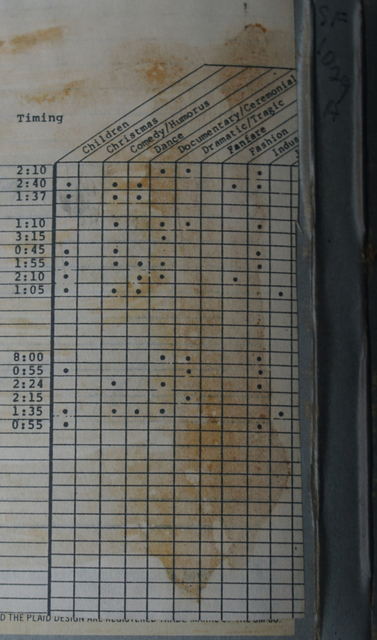
\includegraphics[width=0.6\textwidth]{img/Fig1.jpg}
\alt{The image shows parts of the back cover of a tape recording. In a table, every track (not displayed) is augmented by timing information and whether or not it can be classified as, for example, music for children, comedy, documentary, dramatic/tragic, fashion or industry.}
\caption{Fig. 1: Track classification on a tape}
\end{figure}

While composers aimed for musical diversity, the gender representation
was rather less diverse. Creators were often white men -- with few
exceptions. While library music is usually instrumental only, Barbara
Moore\footnote{The musicians Lorraine Bowen and Sarah Angliss gathered
  material (including a discography) on Barbara Moore -- \enquote{a
  composer, arranger and vocalist who worked in film, television and
  radio}, see \url{https://www.barbaramoore.co.uk/}.} is known for her
recording \enquote{Vocal Shades and Tones} on de Wolfe. Delia Derbishire
experimented with recorded sounds, this approach to composition is also
known as \enquote{Musique concrète}.\footnote{The charitable
  organization \enquote{Delia Derbyshire Day} provides detailed
  information on the musician, see
  \url{https://deliaderbyshireday.com/}. For more information on
  \enquote{Musique concrète} see
  \url{https://en.wikipedia.org/wiki/Musique_concr\%C3\%A8te}.} She was
employed by a library music publisher and later by the BBC for their
\enquote{Radiophonic Workshop}.\footnote{The Radiophonic Workshop was
  initiated to provide the BBC with electronic sounds for their diverse
  broadcasting needs. For more information see the blog
  \url{https://www.soundonsound.com/people/story-bbc-radiophonic-workshop}
  or entry in the \enquote{History of the BBC}
  \url{https://www.bbc.com/historyofthebbc/100-voices/pioneering-women/women-of-the-workshop}.}
There, she and others provided the BBC with themes, jingles and sound
designs. In 1963 they created, for example, the memorable theme of the
long-running TV series \enquote{Dr.~Who}. Derbyshire is an acknowledged
sound pioneer and fulfilled \enquote{the industry's desire to
incorporate sounds from the furthest vanguard of musical
experimentation} (Hollander p.~100).

It's not fully known how many female composers created library music
because of the use of non-female pseudonyms.\footnote{See the article
  \enquote{\enquote*{Madri Dell'Invenzione} Meets \enquote*{La Donna
  Invisibile:} Ten Unsung Italian Library Music Composers. A breakdown
  of the female forerunners of the experimental library music
  metropolis} by Andy Votel,
  \url{https://daily.redbullmusicacademy.com/2019/08/italian-female-library-music-composers}.}
These were used for reasons such as xenophilia\footnote{In one of
  Orlandi's soundtrack compositions she was \enquote{credited with the
  pseudonym Joan Christian. That was a judgement call, because producers
  were infected with xenophilia at that time} (as documented on the back
  cover of her record \enquote{A Doppia Faccia},
  \url{https://www.discogs.com/release/14869649-Nora-Orlandi-A-Doppia-Faccia/}).}
or marketing (see section below).

Walter Carlos -- who later became Wendy Carlos -- was an early
electronic music pioneer who helped improve the Moog synthesizer and
composed some work for TV ads. She is best known for her commercially
successful electronic interpretation of Bach music \emph{(Switched on
Bach)}, and her work as an soundtrack editor or composer for films such
as \enquote{Clockwork Orange}, \enquote{Shining}, and \enquote{TRON}
(1982).\footnote{Villalba, Juanjo (2022): \enquote{Wendy Carlos: The
  brilliant but lonely life of an electronic music pioneer},
  \url{https://english.elpais.com/culture/2022-12-12/wendy-carlos-the-brilliant-but-lonely-life-of-an-electronic-music-pioneer.html}.
  For information on \enquote{Switched on Bach} see
  \url{https://www.discogs.com/master/76226-Walter-Carlos-Switched-On-Bach}.}

Library music is known from Western Europe and the USA. More research
would be needed to document production and usage of such music from/in
other parts of the world.

\hypertarget{metadata}{%
\section{Metadata}\label{metadata}}

Some library recordings were initiated by a \emph{brief} -- a wishlist
by a label representative which usually had bullet-points of moods that
should be achieved. At other times there was no brief and the producer
was free to guess or experiment what would be appreciated by a future
audience.

The recordings were then enriched with metadata that should help
potential users select the appropriate track right away. The genre,
intended mood, tonality, instruments, tempo were at times presented more
prominently than the artist.

Metadata like tempo is also popular in dance music with bpm (beats per
minute); instruments mentioned (associated with certain moods) also
appear on jazz or rock records. Other metadata like tonality is known
from classic recordings. Rather unique to library music are the mood
descriptions. These were sometimes translated/printed in several
languages to reach an even greater audience. The LP \emph{Selected Sound
9015} included English, German, French, Italian and Spanish and we
reproduce an example description for one of the numbered tracks:

\begin{quote}
\enquote{SL 585 Action Shuffle (Berry Lipman / Selected Sound) Beat
Shuffle; dance orchestra with girl's voice; Drive, happy, swinging.
Sports, Journey, young people gathering, airport, big city.
2'47}\footnote{See images of the record cover at
  \url{https://www.discogs.com/release/2728337-The-Sound-Of-Berry-Lipman-Band-Lets-Talk-About-Music}.}
\end{quote}

\begin{figure}
\centering
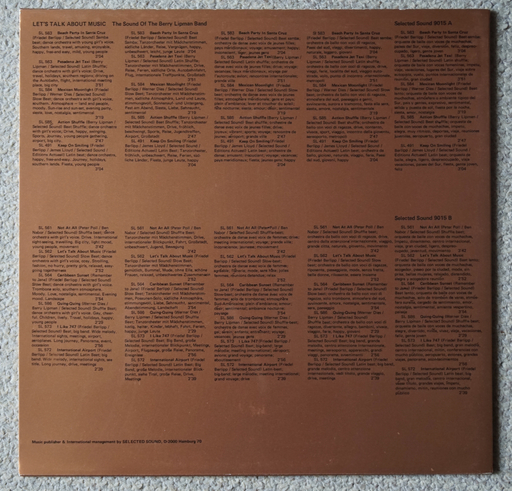
\includegraphics[width=0.5\textwidth]{img/Fig2.jpg}
\alt{The image shows the golden back cover of the vinyl record
Selected Sound 9015. The whole backside is covered in metadata for each
of the numbered tracks, in particular dance type, mood and length. Each
description is translated to four other languages.}
\caption{Fig.~2: Vinyl back cover of 'Selected Sound 9015' with descriptions in 5 languages}
\end{figure}

Some labels even allowed customers to scribble down their own notes in a
dedicated column -- \enquote*{your notes} on \enquote*{MP2000} records
or next to the \enquote*{tempo} descriptions on \enquote*{Tele Music}
productions as shown in Figure 3.

\begin{figure}
\centering
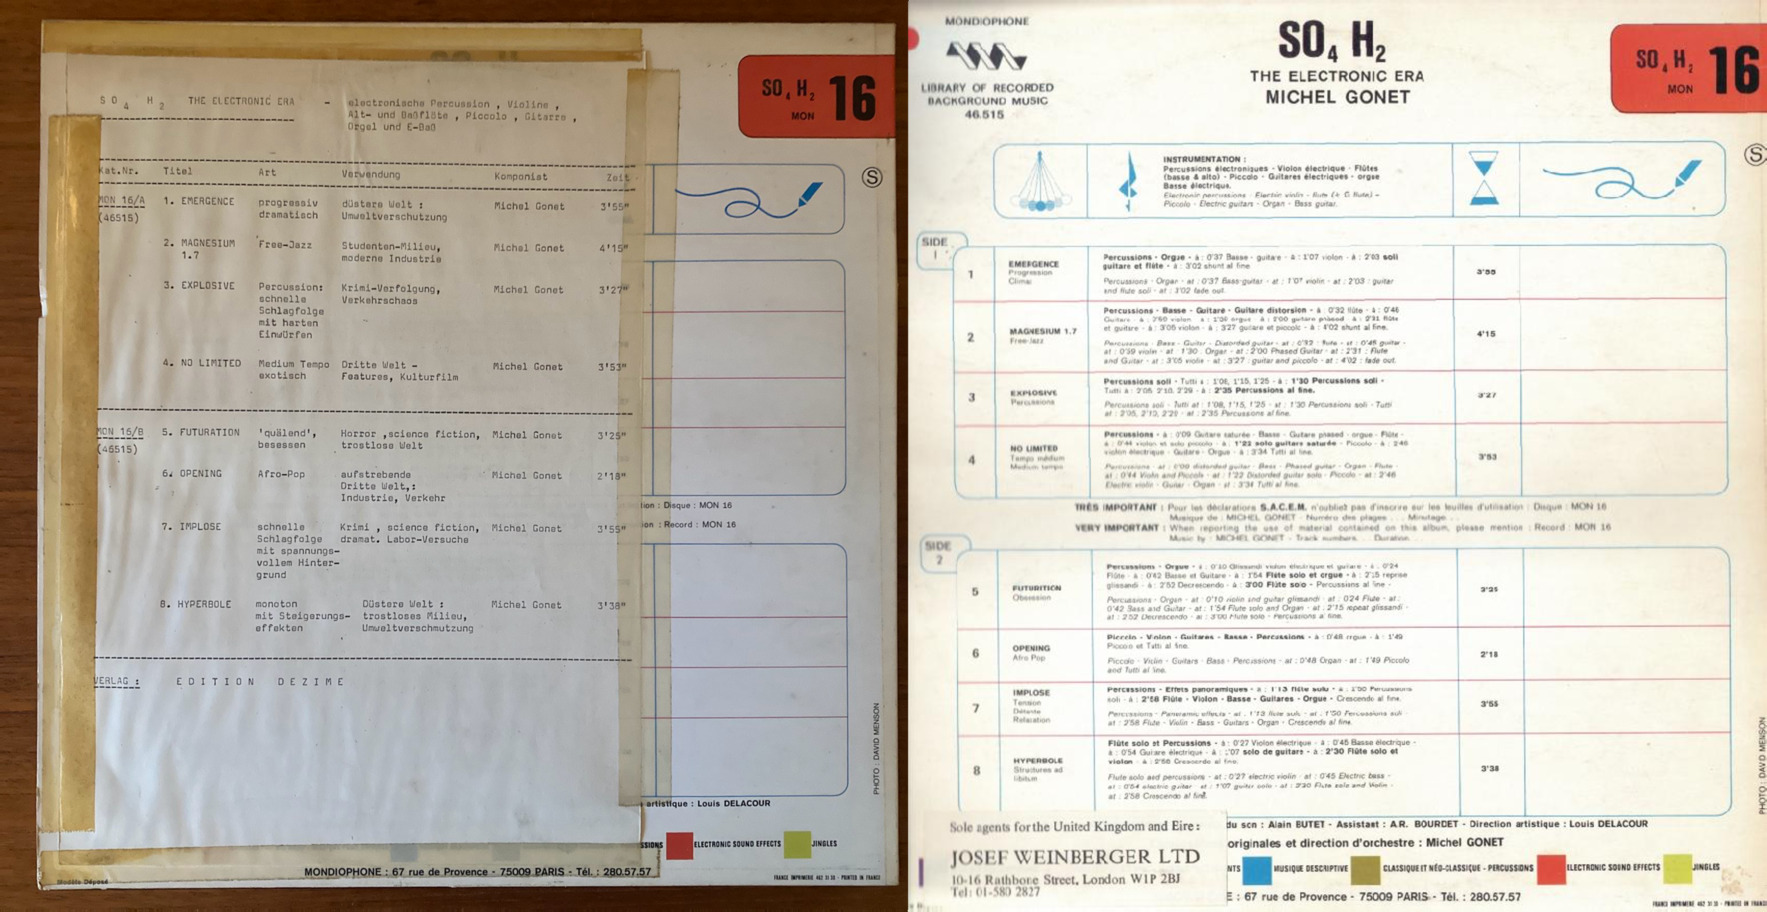
\includegraphics[width=0.8\textwidth]{img/Fig3.jpg}
\alt{The image shows the back cover of a library music record where
the French and English metadata was replaced by a typewriter printout
augmented with mood classification and use case. The column for taking
notes is still visible and untouched. At the bottom and top right, mood
classification in color code is visible for faster retrieval.}
\caption{Fig.~3: Vinyl back cover of Michel Gonet – SO4 H2 The Electronic Era (\url{https://www.discogs.com/release/1112157}) – original on the right; on the left with translated and extended metadata by the former record owner. S/he decided to replace French and English data on instruments and timing with German mood classification and use cases. The notes column and color code classification (bottom and top right) are still visible.}
\end{figure}

Other metadata is provided to increase production value, for example
information on possible cuts or edits as found on James Clarke
\emph{Mystery Movie}\footnote{James Clarke's \enquote{Mystery Movie} was
  published by Themes International (TIM 1015), see
  \url{https://www.discogs.com/release/12577800-James-Clarke-Mystery-Movie/}.}:

\begin{itemize}

\item
  \enquote{Heavy driving movement. Good cutaway points.}
\item
  \enquote{Fast shaker rhythm with electric piano effects. Shock entry
  of guitar at 1.10, builds up to climax and let down to end. Possible
  edit 1.10 to 1.46.}
\end{itemize}

Some labels characterize the whole recording with a set of keywords.
That is sometimes accompanied by track mood descriptions. In other
cases, descriptive titles must suffice. One example for LP and track
mood descriptions can be found on the recording \emph{The Big Beat} by
the label KPM\footnote{\emph{The Big Beat} by composers Keith Mansfield
  and Alan Hawkshaw (published 1969 by KPM), see
  \url{https://www.discogs.com/master/80755-Keith-Mansfield-Alan-Hawkshaw-The-Big-Beat/}.}:

\begin{itemize}
\item
  \enquote{Pounding -- Thumping -- Rocking -- Pulsating}
\end{itemize}

This helps the user to narrow down a search for the right mood. But not
all labels take advantage of elaborate metadata. Some labels only used
record and/or track titles.

The KPM 1157 LP \enquote{The Hunter (Drama Suite) / Adventure Story} is
an example for extensive metadata, as it provides descriptive track
names, length and also remarks for the potential sound(track)
editor\footnote{\emph{The Hunter (Drama Suite) / Adventure Story} was
  published in 1975 by KPM and compiles works by different composers,
  see
  \url{https://www.discogs.com/master/1653869-Various-The-Hunter-Drama-Suite-Adventure-Story}.}:

\begin{itemize}

\item
  \enquote{Heavy Lead (1:43) Menacing underlying movement.}
\item
  \enquote{Uneasy Silence (2:05) Static underlying tension--solo bass
  flute}
\item
  \enquote{Battle (1:00)}
\end{itemize}

On this LP, some tracks are produced to be combined or used as
alternatives for different effects. Certain remarks represent additional
value for the editor making this record more useful in soundtrack
production:

\begin{itemize}

\item
  \enquote{Hideout (2:55) \emph{Suspended tension. Build to tail end.}}
\item
  \enquote{Hideout---shock (0:05) \emph{Shock chord (as alternative to
  end).}}
\item
  \enquote{Hideout---let down (0:12) \emph{Build to let down (as
  alternative end).}}
\end{itemize}

The Austrian library music composer Gerhard Narholz remembers that such
metadata can be challenging to create:

\begin{quote}
\enquote{I'm really running out of titles sometimes. Because in Germany,
we have over 300,000 tracks in the library. And the number of suitable
words to describe music is limited. So it's not easy sometimes.}
(Narholz as quoted in Hollander p.~151)
\end{quote}

On the record \emph{Slow}\footnote{See image of the back cover for
  \emph{Slow} at
  \url{https://www.discogs.com/master/3294286-Various-Slow-Motion-And-Movement}.}
he chose to differentiate similar compositions by numbers, for example:

\begin{itemize}
\item
  \enquote{Deja Vu 1}
\item
  \enquote{Deja Vu 2}
\end{itemize}

Classifying such music is futile as it is produced to cover all genres.
Unsurprisingly, the few records that appear in record shops lack their
own category and are at times filed under \emph{Soundtracks}, or
\emph{Easy Listening}.

Certain production music labels attempted to provide classification
information on the front cover that could be beneficial for filing away
the media or maybe finding it faster when browsing through the library.
This is exemplified in Figure 4.

\begin{figure}
\centering
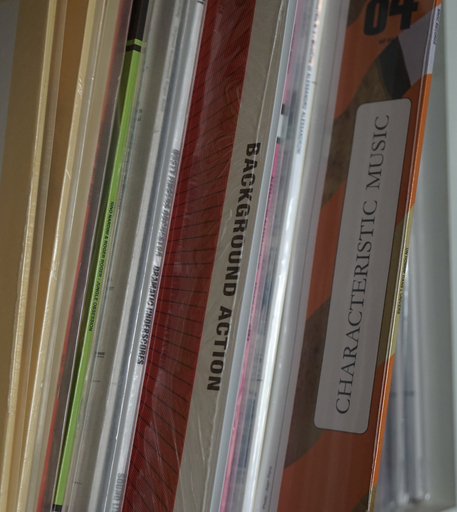
\includegraphics[width=0.6\textwidth]{img/Fig4.jpg}
\alt{The image shows record covers on a shelf with classification
information printed in large font prominently on the side of the cover.}
\caption{Fig.~4: Strategically placed metadata on LP cover}
\end{figure}

Assigning metadata like keywords is non-trivial. A movie producer
searching for library music mentioned in a private conversation with us
that certain online platforms suffer from keyword spamming and that
user-provided keywords were not always helpful, lacking specificity. But
some stock music platforms provide waveform visualization which helps
him in selecting tracks for further investigation.

Other visual information from recordings include the differently shaped
sections of the groove pressed into the vinyl, depending on actual music
dynamics. On master tapes, library producers left pauses in between
tracks to ease editing the tape.

\begin{quote}
\enquote{And if you didn't do this, the editor might love your music,
but just doesn't got time to work out an ending, so he's going to go for
something else} (Mansfield as quoted in Hollander p.~41)
\end{quote}

\hypertarget{covers}{%
\subsection{Covers}\label{covers}}

Some record covers were produced by the artists themselves, others by
labels. They exhibit a variety in designs owed to the restricted
resources, sometimes resulting in wildly artistic endeavors:

\begin{quote}
\enquote{The same brief seems to have been given to the sleeve designers
as to the musicians -- \enquote*{zero budget and complete and utter
artistic freedom to indulge in your most disturbed inner fantasies}.}
(Dammers in foreword to Trunk p.~9)
\end{quote}

Some library music covers exhibit a recognizable minimalistic design.
The green KPM 1000 series lacks additional metadata on the front cover.
For some issues, the de Wolfe label chose red covers with minimalistic
black logo and typography. The \enquote*{Library Music} edition
\enquote*{April Orchestra} uses a particular typography with a different
color for each recording. Cataloging recording series is sometimes
challenging.\footnote{As an example, see the entry in the
  \enquote{profile} field of the following database entry, pointing out
  that \enquote*{April Orchestra} is not the artist, see
  \url{https://www.discogs.com/label/52749-April-Orchestra?page=1}.}
While the \enquote*{April Orchestra} series only mentions the composer,
the \enquote*{Tele Music} cover just shows the title.

\begin{figure}
\centering
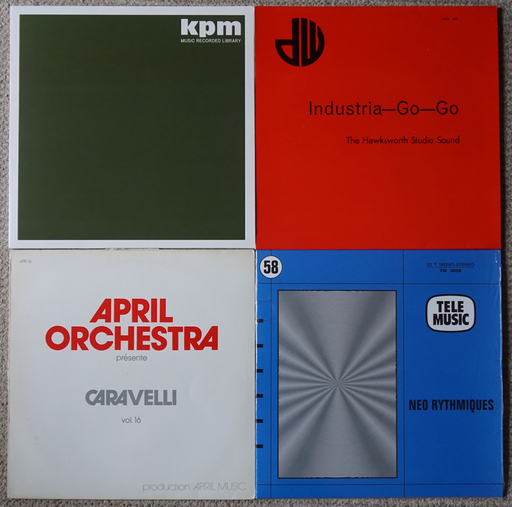
\includegraphics[width=0.6\textwidth]{img/Fig5.jpg}
\alt{The image shows four record covers in different colors with
minimalistic typography}
\caption{Fig.~5: Four minimalistic library music covers}
\end{figure}

While we can only provide few examples of cover art here, publications
like Trunk\footnote{Trunk, Jonny (2016): The Music Library. London: Fuel
  design \& Publishing, Revised and expanded edition. (ISBN:
  978-0-9931911-3-8)} and Hollander\footnote{Hollander, David (2018):
  Unusual Sounds. New York: Anthology Editions. (ISBN:
  978-1-944860-12-7)} are dedicated to the various cover artwork of
library music releases. Jonny Trunk also discusses a small selection of
such covers online.\footnote{Selection of ten of Jonny Trunk's favorite
  library music albums, see
  \url{https://www.thewire.co.uk/galleries/gallery_the-music-library}.}
Unfortunately, artistic effort decreased during the advent of the CD due
to its smaller size (Narholz in Hollander p.~153~f).

\hypertarget{economics}{%
\section{Economics}\label{economics}}

\hypertarget{history}{%
\subsection{History}\label{history}}

Early silent movies were sometimes underscored live by a piano or organ
player. One of the earliest labels producing music for such cinematic
events was \enquote{Music de Wolfe} which started releasing music for
\enquote*{synchronizing} films in 1927. Over the decades, several media
types were utilized: Early recordings were pressed as 10'' records --
played at 78 rpm (rounds per minute). Later, 33 rpm 12'' vinyl was used
for LPs and a few smaller 45 rpm 7'' records were pressed as well,
likely for promotion. Both formats are still playable on modern record
players. The development continued to CDs and, nowadays, digital online
media.

The increasing production of films and TV programs starting in the 1950s
and 60s required far more music and \emph{cues}, which could be
characterized as short sounds. Not every production could hire a
dedicated composer and welcomed pre-existing productions:

\begin{quote}
\enquote{With any new programme, producers on a budget have limited
options. To commission a new theme is expensive, so it makes economic
sense to use the mood music library and instantly access a wealth of
well played, potentially suitable music.} (Trunk p.~7)
\end{quote}

Cover versions of popular songs were produced and made hit melodies
cheaply available for (re)use. A scene of competing music producers
developed that recorded such productions. The music was sent
speculatively to potential users in film, TV and radio. (Neil Brand in
\emph{BBC The Sound of TV} -- Theme Tunes)\footnote{\enquote{Neil
  Brand's Sound of TV} (TV documentary series, BBC, 2020), episode.
  \enquote{Theme Tunes} \url{https://www.imdb.com/title/tt13612792}}

Production value characterizes library music. It has to deliver a mood
to the point in seconds. Such a production style made it useful for a TV
ad, jingle or similar. And the sound had to be right on the first take,
because there were so many recordings to make and so many other
musicians willing to play.

\hypertarget{marketing}{%
\subsection{Marketing}\label{marketing}}

From a librarian's point of view, library music could in parts be
compared with \enquote*{grey literature}: Not available on the open
market but retrievable by or offered to interested parties like creators
of sound tracks, news programs and so on.

Selected recordings were made available to sound editors as a vocal and
instrumental record, which allows cutting between the two versions, for
example, \enquote{The Voice of Soul} and \enquote{The Sound of Soul}
(Hollander p.~103).\footnote{\enquote{The Voice Of Soul} by Alan Parker
  and Madeline Bell, see
  \url{https://www.discogs.com/master/1429214-Alan-Parker-Madeline-Bell-The-Voice-Of-Soul}.
  \enquote{The Sound Of Soul} by various artists, see
  \url{https://www.discogs.com/master/1429531-Various-The-Sound-Of-Soul}.}
A few records were also released as library and commercial versions. For
example, Tony Newman's \enquote{Soul Thing} is very similar to Keith
Mansfield's \enquote{Funky Fanfare}.\footnote{\enquote{Soul Thing} by
  Tony Newman (1968), see
  \url{https://www.discogs.com/master/585423-Tony-Newman-Soul-Thing}.
  The track \enquote{Funky Fanfare} was released on the compilation
  \enquote{Beat Incidental} (by Alan Hawkshaw and Keith Mansfield,
  released 1969), see
  \url{https://www.discogs.com/master/1441172-Alan-Hawkshaw-Keith-Mansfield-Beat-Incidental}.}
The latter tune has also been used as background music for a visual
snippet which decades later has been reused by Quentin Tarantino and
Robert Rodriguez as part of the intro sequence of some
movies.\footnote{See the visual snippet
  \url{https://www.youtube.com/watch?v=MOwGBzbXb8k} (created by the
  \enquote{National Screen Service} in 1968) and read more about the
  origin and different use cases at
  \url{https://company-bumpers.fandom.com/wiki/Astro_Daters/Grindhouse_Bumpers}.}

Marketing considerations are also apparent on some record covers, see
the example for Oronzo de Filippi. The artists are less important than
the usability for the target audience -- the sound editor -- which are
reflected in visual art that at best transports certain moods.

\begin{quote}
\enquote{There are no pictures of {[}the musicians{]} on the record
sleeves, no personality cult, no fashion, no looks or age to confuse
things. Another plus is that not a note of this music was ever played
live, or sold directly to the public, so irrelevant irritations like
audience reaction or \enquote*{commercial viability} weren't really a
consideration.} (Dammers in foreword to Trunk p.~8)
\end{quote}

\begin{figure}
\centering
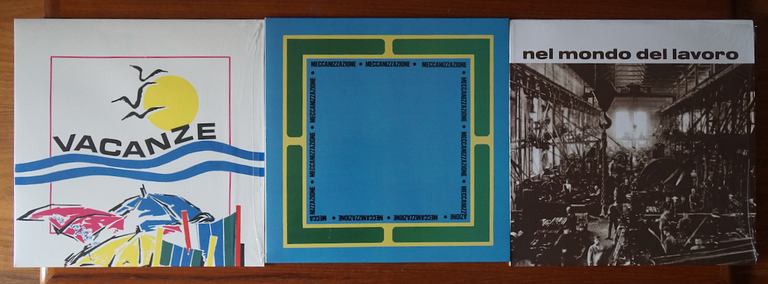
\includegraphics[width=1\textwidth]{img/Fig6.jpg}
\alt{The image shows three record covers for the artist Oronzo de
Filippi. The left is titled \enquote*{Vacanze} and shows a stylized
beach scene on a white background. The record in the middle is titled
\enquote*{Meccanizzazione} inside a large square on a blue background.
The cover to the right shows a black and white scene from a factory
floor and the title \enquote*{Nel Mondo Del Lavoro}.}
\caption{Fig.~6: Three example covers for library music composer Oronzo de Filippi, only the titles are displayed on the front: \enquote*{Vacanze}, \enquote*{Meccanizzazione}, \enquote*{Nel Mondo Del Lavoro}}
\end{figure}

Marketing included playing music for clients in person, because vinyl
records exposed some crackles and noise -- not helpful in selling rights
to certain music. Listening to (master) tapes was offered as well
(Narholz in Hollander p.~151).

Some marketing strategies are common in the music business. A record
distributor would describe the media briefly in a catalog, a fellow
artist may have been tasked to write a commentary printed as liner notes
on the back. The musicians/producers/composers would give each track a
remarkable (or descriptive) name and add notes about, for example, tempo
and instruments. In addition to that, library music also received
information about the atmosphere or mood. Today, library music is at
times also marketed by who sampled the records or catalog.\footnote{Daniel
  Sanchez mentions some popular music artists who sampled library music
  distributed by the label KPM, see
  \url{https://www.digitalmusicnews.com/2019/01/16/sony-atv-emi-kpm-music-library}.}
The label KPM was also rebranded to revive its old household
name.\footnote{KPM was founded in 1960 as an independent label, acquired
  by the major label EMI in 1969, and rebranded to EMI Production Music
  in 2011. In 2021, EMI (since 2018 subsidiary of Sony Music) announced
  \enquote{EMI Production Music has returned to its flagship brand name
  KPM Music}, see
  \url{https://www.sonymusicpub.com/en/news/3331/emi-production-music-rebrands-to-kpm-music}.}

The music itself also works as a marketing tool and helped composers to
get into movie or TV music business -- as an example (and mentioned
before), the theme music for the Netflix series \enquote{Stranger
Things} was born as a library recording.\footnote{See the interview with
  the Band \enquote{Survive} whose career was boosted exceptionally
  after having contributed the score,
  \url{https://www.billboard.com/music/rock/survive-stranger-things-soundtrack-interview-7488050/}.}

Library music labels encouraged their composers/musicians to take on
pseudonyms/aliases. Otherwise a single composer would have been
mentioned on 20--30 records which was assumed to deter potential buyers.
Most producers are secretive about it as it allowed them to get more
music into the market (to be reused). Some composers are said to have
tens of thousands of records under several names (Hollander p.~27).
Others used pseudonyms to bend rules as their artist names were likely
contracted to a publisher. Some composers used different names because
the audience was assumed to be biased to believe that if some composer
could write classical music, they could not write a jazz piece or dark
tune (Narholz in Hollander p.~151).

\hypertarget{rights-and-licensing}{%
\subsection{Rights and Licensing}\label{rights-and-licensing}}

The Music Union in the UK required each and every track recorded to be
enriched with metadata like who and when it was recorded in order to get
royalties whenever it was (re)used (Kerridge in Hollander p.~34). This
at times conflicted with the hire-for-money approach to such music
productions and the intended rights ownership. As a consequence, London
based labels like \enquote{Themes} had most of their sessions recorded
in Germany (Trunk p.~226). (In parts, because German recording engineers
had the reputation to be \enquote{very correct} (Kerridge in Hollander
p.~37).)

The story goes that one of the Beatles convinced Michael Jackson to buy
music rights, who then decided to buy the rights to the Beatles music.
Michael Jackson is also said to have bought the rights for the library
label Bruton music (and probably others). Handling music rights
continues to be a lucrative business.\footnote{For example, the major
  music label BMG and the streaming platform Netflix have entered a long
  term agreement for the (exclusive) management and administration of
  Netflix's music publishing rights, see
  \url{https://www.bmg.com/de/news/Netflix-BMG-new-exclusive-music-deal.html}.}

Some labels disposed of their old stock of library music when its
perceived usefulness decreased. That's how some of the vinyl became
available to the general public -- an opportunity some record collectors
jumped on. At the same time, recordings -- made available to prospective
users and/or later discarded -- must not be re-sold. So, discarded dead
stock appearing on online auction platforms is only currently tolerated
(Hollander p.~30).

Once digitization is done, it becomes easier to \enquote{request a
synchronization license}, see for example the platform
\url{https://secondhandsongs.com} where the concept is explained as:

\begin{quote}
\enquote{A synchronization license allows you to use the work with some
kind of visual media output (film, television shows, advertisements,
video games, accompanying website music, movie trailers,
etc.).}\footnote{See for example The Charmels' song \enquote{As long as
  I've got you}: mouse-over the question mark for entry \enquote{Request
  a synchronization license} at
  \url{https://secondhandsongs.com/performance/145209/all}}
\end{quote}

\hypertarget{experiments}{%
\subsection{Experiments}\label{experiments}}

Some argue that due to the economic situation, composers were asked to
produce a lot of music. They were given freedom to experiment, and they
did so (Parker in Hollander p.~49).

\begin{quote}
\enquote{The {[}coloursound{]} label's catalog {[}\ldots{]} now stands
as a tribute to the unfettered creative license that libraries were able
to provide to their forward-thinking musicians who, frustrated by the
whims and constraints of the commercial scene, found complete freedom in
the world of production music.} (Hollander p.~156)
\end{quote}

These were talented composers, often building their own studio or maybe
being invited to some label's studio. Some of the composers experimented
heavily with unusual instruments like the harpsichord or later analog
synthesizers which is reflected in the relationship to \enquote{Musique
Concrète}.

TV testcards -- originally not meant to be seen by the general public
but displayed throughout the program at certain times -- received their
own musical treatment and library music labels issued something as
background. It may have been Easy Listening or Jazz if it was not the 10
min sinus tone. Technically not library music, testcard music also
attempted to create moody atmospheres on a channel that had nothing else
to show.

\hypertarget{session-musicians}{%
\subsection{Session Musicians}\label{session-musicians}}

Writers and producers shared most of the rights and profits. The actual
musicians were hardly credited, as they were mostly thought to be
replaceable. They were paid after the session (Narholz in Hollander
p.~151) and usually saw no royalties from the recordings. Session
musicians were used in many other genres and recordings to the same
effect. Some groupings became well-known and were in-demand in the
recording industry.\footnote{Popular session musician groups were for example \enquote{The Wrecking Crew}(\url{https://www.imdb.com/title/tt1185418/}) or \enquote{The Funk Brothers} (\url{https://www.imdb.com/title/tt0314725}). Others are discussed in the \enquote{Library Music Film}, \url{https://www.imdb.com/title/tt24510110/}.}

\hypertarget{recommendations-for-further-readingwatching}{%
\section{Recommendations for Further
Reading/Watching}\label{recommendations-for-further-readingwatching}}

Articles and Books:

\begin{itemize}
\item
  Nate Patrin (2014) \enquote{The Strange World of Library Music},
  \url{https://pitchfork.com/features/starter/9410-library-music/}
\item
  Jonny Trunk (2019) \enquote{The What, How and Why of Library Music},
  \url{https://daily.redbullmusicacademy.com/2019/08/the-what-how-and-why-of-library-music}
\item
  Adrian Kerridge (2016) \enquote{Tape's rolling, take one!},
  {[}Hertford{]} : M-Y Books, digitized book via
  \url{https://archive.org/details/tapesrollingtake0000kerr}
\end{itemize}

Documentaries (video or audio):

\begin{itemize}
\item
  \enquote{Library Music Film}: 2018 documentary by Paul Elliott and
  Sean Lamberth (113 min), \url{https://www.imdb.com/title/tt24510110/};
  extended teaser (5:08 min)
  \url{https://www.youtube.com/watch?v=RgOMibjOJcw}
\item
  Trailer (6:40 min) marketing the \enquote{Unusual Sounds} publication:
  \url{https://www.youtube.com/watch?v=-2CgmA0-X-U}
\item
  Jonny Trunk (2011) \enquote{Into the Library}, BBC radio program,
  \url{https://www.bbc.co.uk/programmes/b01061hr}
\item
  \enquote{Sisters with Transistors}: 2020 documentary (126 min) by Lisa
  Rovner, \url{https://www.imdb.com/title/tt6744250}
\end{itemize}

Audio Mix of different library music recordings:

\begin{itemize}
\item
  Library Music Mix (54 min)
  \url{https://soundcloud.com/djslingshot/walking-in-the-dark-library-music-45s-vol-1}
\end{itemize}

\hypertarget{references}{%
\section{References}\label{references}}

\enquote{Neil Brand's Sound of TV} (TV documentary series, BBC, 2020),
episode \enquote{Theme Tunes}
\url{https://www.imdb.com/title/tt13612792}

\enquote{Neil Brand's Sound of TV} (TV documentary series, BBC, 2020),
episode \enquote{Advertising and Jingles}
\url{https://www.imdb.com/title/tt13630856}

Hollander, David (2018): Unusual Sounds. New York: Anthology Editions.
(ISBN: 978-1-944860-12-7)

Trunk, Jonny (2016): The Music Library. London: Fuel design \&
Publishing, Revised and expanded edition. (ISBN: 978-0-9931911-3-8)

%autor
\begin{center}\rule{0.5\linewidth}{0.5pt}\end{center}

\textbf{Alexander Struck} has a background in Library \& Information
Science as well as Computer Science. He worked in the publishing
industry and later on problems of network analysis. For the past decade
Alexander has been the CTO/CIO of Clusters of Excellence, currently
``Matters of Activity. Image Space Material''
\url{https://ror.org/05tbc9841}. He published on research software,
hardware and evaluation: \url{https://orcid.org/0000-0002-1173-9228}.
For the past decades, Alexander has been collecting records from diverse
genres.

\end{document}